%In this section we discuss how the Provenance Data Model interacts with
%classes and attributes from other VO data models (especially DatasetDM).
%(e.g. DatasetDM, SpectralDM (share some same classes), SimDM) 
%and how provenance information can be stored.

The Provenance Data Model can be applied without making any links to other 
IVOA data model classes. For example, when the data is not yet published, provenance information
can be stored already, but a DatasetDM-description for the data may not yet exist.
However, if there are data models implemented for the datasets, then it is 
very useful to connect the classes and attributes of the other data models with Provenance classes and attributes (if applicable), which we are going to discuss in this Section. These links help to avoid 
unnecessary repetitions in the metadata of datasets, and also offer the possibility 
to derive some basic provenance information from existing data model classes automatically.


\subsection{Links with Dataset/Obscore Model}
\label{sec:dataset-obscore}

Entities and their descriptions in the Provenance Data Model 
are tightly linked to the \class{DataSet}-class in the DatasetDM/ObsCore Data Model, as well as to 
InputDataset and OutputDataSet in the Simulation Data Model \citep[SimDM,][]{std:SimDM}.
Table \ref{tab:datasetmapping} maps classes and attributes from DatasetDM
to concepts in the Provenance Data Model.


%\begin{figure}[h]
%\centering
%\includegraphics[width=\textwidth]{../datamodel-diagrams/images/classes-relations-dms}
%\caption{Links between Agent and Party, Entity and Dataset.}
%\label{fig:class-relations-dm}
%\end{figure}
% --> a similar figure is already given in the sections on entity and agent.

\begin{table}[h]
\small
\tymax  0.5\textwidth
\begin{tabulary}{1.0\textwidth}{@{}Llp{5cm}@{}}
\toprule
\head{ProvenanceDM} & \head{DatasetDM} & \head{Comment}\\
\midrule
Entity.id                & Curation.PublisherDID  & unique identifier for the dataset assigned by the publisher\\
Entity.id                & DataID.creatorDID      &  alternative id for the dataset given by the creator, could be used as Entity.id if no PublisherDID exists (yet)\\
Entity.name              & DataID.title           & title of the dataset\\
Entity.rights            & Curation.Rights        & access rights to the dataset; one of [...]\\
Entity.creationTime      & DataID.date            & date and time when the dataset was completely created\\
HadMember.collection     & DataID.collection     & link to the collection to which the dataset belongs\\
WasGeneratedBy.activityId & DataID.ObservationID  & identifier to everything describing the observation\\
Agent                    & Curation.Contact       & link to Agent with role contact\\
Agent.id                 & Curation.PublisherID   & link to the publisher, i.e. to an Agent with role=``publisher''\\
Agent.name, \newline wasAttributedTo.role=\newline Creator               & DataID.creator         & name of agent creating the dataset\\
Agent.name, \newline wasAttributedTo.role=\newline Publisher               & Curation.Publisher     & name of the publisher\\
\midrule
\multicolumn{3}{c}{\bf Attributes specific to dataset entities}\\
\midrule
Entity.releaseDate       & Curation.Date          & release date of the dataset\\
Entity.version           & Curation.Version       & version of the dataset\\
Entity.reference         & Curation.Reference     & link to publication\\
EntityDescription.dataproduct\_type & DataProductType & the type of a dataproduct from DatasetDM can be used as attribute to EntityDescription\\
EntityDescription.dataproduct\_subtype & DataProductSubType & subtype of a \mbox{dataproduct}/entity\\
EntityDescription.calibLevel & ObsDataset.calibLevel & (output) calibration level, integer between 0 and 3\\
\bottomrule
\end{tabulary}
\caption{Mapping attributes from DatasetDM classes to (optional) attributes in ProvenanceDM. Attributes like \emph{EntityDescription.calibLevel} are very specific to entities described with DatasetDM and thus are not included in Table~\ref{tab:entitydescription-attributes} for \emph{EntityDescription}. }
\label{tab:datasetmapping}
\end{table}


\begin{figure}[h]
\centering
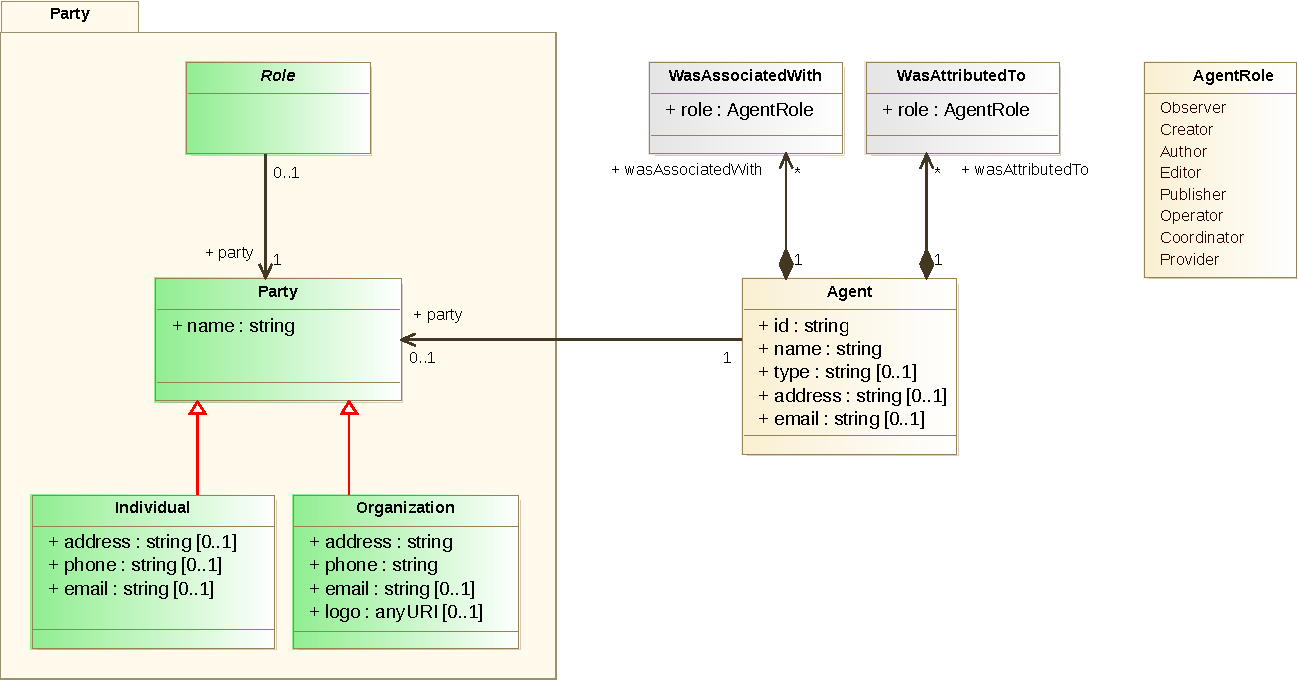
\includegraphics[width=\textwidth]{../datamodel-diagrams/images/agent-relations.pdf}
\caption{The relations between the \class{Agent} class within ProvenanceDM 
(grey and yellow classes) with classes from the DatasetDM, party package (green).}
\label{fig:agent-relations}
\end{figure}

The \class{Agent} class, which is used for defining responsible persons and 
organizations in ProvenanceDM, is very similar to the \class{Party} class in DatasetDM (and in SimDM). Its details are depicted in Figure~\ref{fig:agent-relations}.
The main difference between \class{Agent} and \class{Party} is that \class{Individual} and \class{Person} are subclasses in DatasetDM, whereas we just use the same class \emph{Agent} for both and distinguish between them using the \emph{Agent.type} attribute (which can have the value ``Individual'' or ``Organization''), which is closer to W3C's provenance data model.
% Which is closer to W3C ProvDM!


We imagine that services implementing both data models, \class{Dataset} and \class{ProvenanceDM} may just use \emph{one} class: either \class{Agent} or \class{Party}, enriched with all the necessary (project-specific) attributes. When delivering the data on request, the serialised versions can be adjusted to the corresponding notation.
Note that for Provenance queries using a ProvTAP service or for W3C compatible serializations, the name \class{Agent} for the responsible individuals/organizations is required.



\subsection{Links with Simulation Data Model}
In SimDM one also encounters a normalization similar to our separation of descriptions from 
actual data instances and executions of processes: the SimDM class ``experiment'' 
is a type of \class{Activity} and its general, reusable description is called a ``protocol'',
which can be considered as a type of this model's \class{ActivityDescription}. 
More direct mappings between classes and attributes of both models are given in Table~\ref{tab:simdmmapping}.

\begin{table}[h]
\small
\tymax  0.5\textwidth
\begin{tabulary}{1.0\textwidth}{@{}Llp{5cm}@{}}
\toprule
\head{ProvenanceDM} & \head{SimDM} & \head{Comment}\\
\midrule
Activity               & Experiment      &  \\
Activity.name          & Experiment.name & human readable name; name attribute in SimDM is inherited from Resource-class\\
Activity.endTime & Experiment.executionTime  & end time of the execution of an experiment/activity \\
Activity.description & Experiment.protocol & reference to the protocol or ActivityDescription class \\
ActivityDescription    & Protocol        & \\
ActivityDescription.name  & Protocol.name   & human readable name\\
ActivityDescription.doculink & Protocol.referenceURL & reference to a webpage describing it\\
% add Protocol.code, Protocol.version?
Parameter              & ParameterSetting     & value of an (input) parameter\\
ParameterDescription   & InputParameter       & description of an (input) parameter\\
Agent           & Party           & responsible person or organization\\
Agent.name      & Party.name      & name of the agent \\
WasAssociatedWith & Contact         & classes for linking to agent/party\\
WasAssociatedWith.role & Contact.role    & role which the agent/party had for a certain experiment (activity); SimDM roles contain: \texttt{owner}, \texttt{creator}, \texttt{publisher}, \texttt{contributor}\\
WasAssociatedWith.agent & Contact.party    & reference to the agent/party \\
Entity        & DataObject     & a dataset, which can be/refer to a collection\\

\bottomrule
\end{tabulary}
\caption{Mapping between classes and attributes from SimDM to classes/attributes in ProvenanceDM. This list is not complete.}
\label{tab:simdmmapping}
\end{table}

If simulations are already described with SimDM, this table can be used
to map from SimDM properties to ProvenanceDM, e.g. when serving serialized provenance
metadata via an additional ProvDAL interface or for storing provenance
metadata together with each released simulation dataset (e.g. in a VOTable).

% Remove this, because no further links to other data models are currently planned.
%\subsection{Further links to data models}
%More similarities and links to other data models will be detailed in future
%versions of this working draft.
